\documentclass[10pt,twocolumn]{article}
	
\usepackage{myfontstyle}
\usepackage{mypackages}
\usepackage{mymacros}
\usepackage{mycommands}
\usepackage{graphicx}
\usepackage{hyperref}
\usepackage{listings}
\usepackage{xcolor}


%%% This defines a style for code blocks (listings package) ----------------
\definecolor{codegreen}{rgb}{0,0.6,0}
\definecolor{codegray}{rgb}{0.5,0.5,0.5}
\definecolor{codepurple}{rgb}{0.58,0,0.82}
\definecolor{backcolour}{rgb}{0.95,0.95,0.92}

\lstdefinestyle{mystyle}{
    backgroundcolor=\color{backcolour},   
    commentstyle=\color{codegreen},
    keywordstyle=\color{magenta},
    numberstyle=\tiny\color{codegray},
    stringstyle=\color{codepurple},
    basicstyle=\ttfamily\footnotesize,
    breakatwhitespace=false,         
    breaklines=true,                 
    captionpos=b,                    
    keepspaces=true,                 
    numbers=left,                    
    numbersep=5pt,                  
    showspaces=false,                
    showstringspaces=false,
    showtabs=false,                  
    tabsize=2
}

\lstset{style=mystyle}

%%%----------------------------------------

\begin{document}
\thispagestyle{fancy1}

%%% Title and Abstract------------------------
\twocolumn[
\begin{center}
	\hrule
	\vspace{3pt}
	% Title:
	{\sffamily\bfseries\Large
		Report for Laboratory 7: Motor Velocity Control
	} \\
	{\color{gray}
		\vspace{3pt}
		\hrule
		\vspace{3pt}
	}
	{
		\hspace*{\fill}
		Julian Soh
		\hspace*{\fill}
%		Second Author
%		\hspace*{\fill}
%		Third Author
%		\hspace*{\fill}
%		Fourth Author    % uncomment these two lines if there's a fourth author
%		\hspace*{\fill}
	}\\
	\vspace{3pt}
	{\itshape
		\hspace*{\fill}
		Department of Mechanical Engineering, Saint Martin's University
		\hspace*{\fill} \\
		\hspace*{\fill}
		ME/EE 477---Embedded Real-Time Computing for Mechanical Engineers
		\hspace*{\fill}
	}\\
	\vspace{3pt}
	{
		\hspace*{\fill}
		\today{} % today's date ... can type manually instead
		\hspace*{\fill}
	}
	\vspace{3pt}
	{\color{gray}\hrule}
%	\vspace{2pt}
\end{center}
% Abstract:
\begin{adjustwidth}{1.5in}{1.5in}
{\small
\noindent\textbf{Abstract.} \hspace{1em}
This lab implements a program that is a closed-loop control system whereby a motor that is being driven
is measured for (actual) velocity. This velocity is continuously compared to the input (desired) velocity. The difference
between the two velocities is used to compute a control signal that is sent to the motor to adjust its speed, hence
the closed-looped nature of the system. 
}
\end{adjustwidth}
\vspace{9pt}
\hrule
\vspace{1\baselineskip}
]

%%% Body -------------------------

\section{Introduction} 
\label{sec:introduction}
This laboratory exercise focuses on building a motor-speed control application as an integrated closed-loop system. The controller continuously compares the commanded velocity with the measured motor velocity and updates the drive signal in real time to reduce the tracking error. The target closed-loop architecture used in this report is shown in Figure~\ref{fig:SchemaClosedLoop} and follows the framework described by \citet{Picone2024}.

\begin{figure}[htb]
	\centering
	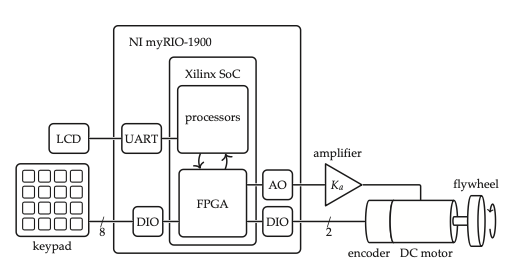
\includegraphics[width=.9\linewidth]{figures/Schema-Closed-Loop.png}
	\caption{Schematic diagram of the target closed-loop system.}
	\label{fig:SchemaClosedLoop}
\end{figure}

The objectives of this exercise were to:
\begin{enumerate}
	\item Integrate the hardware and software components developed in earlier work into a unified closed-loop control system
	\item Implement a program structure that supports continuous adjustment of control parameters without stopping the control algorithm
	\item Implement a proportional-integral (PI) velocity control algorithm for the DC motor
\end{enumerate}

The laboratory procedure, real-time implementation approach, instrumentation context, and supporting theory used in this report are aligned with the course reference material in \citep{Picone2024}.

\section{Materials and Methods}

\subsection{Materials}
The materials used in this experiment were:
\begin{itemize}
	\item Windows 10 computer with myRIO support for C and Eclipse IDE.
	\item NI myRIO-1900
	\item Keypad
	\item Serial display
	\item PMDC motor
	\item Analog current amplifier
	\item DC power supply
	\item Quadrature encoder
	\item Flywheel
	\item Noncontact tachometer
	\item Oscilloscope (optional)\footnote{The oscilloscope was connected to $\mathrm{AO}0$ to monitor the power output from the myRIO for troubleshooting purposes and for further demonstration in Problem L7.5.}
\end{itemize}

\subsection{Main Function Implementation}
The \texttt{main()} routine coordinates initialization, user interaction through the table editor, and orderly shutdown of the timer-driven control thread. Its sequence is:
\begin{enumerate}
	\item Initialize all table-editor variables.
	\item Configure, install, and enable the timer IRQ.
	\item Register and create the timer thread that services the interrupt. For this lab, the thread resource structure includes a pointer to the table data so the ISR-side logic can access current parameters.
	\item Launch the table editor using six entries:
\end{enumerate}

\begin{itemize}
	\item \texttt{V\_R}: rpm \{edit\}
	\item \texttt{V\_J}: rpm \{show\}
	\item \texttt{VDAout}: mV \{show\}
	\item \texttt{Kp}: V-s/r \{edit\}
	\item \texttt{Ki}: V/r \{edit\}
	\item \texttt{BTI}: ms \{edit\}
\end{itemize}

All editable values are initialized to zero, except the BTI setting, which is initialized to $5\,\text{ms}$. After the table editor exits, \texttt{main()} signals the timer thread to stop and then waits until that thread terminates cleanly.

\subsection{Interrupt Service Routine (ISR) Thread}
At the top of the timer-thread entry function, convenient aliases are created for table entries through the table pointer, for example:

\begin{lstlisting}[language=C]
double *Omega_R = &((threadResource->a_table + 0)->value);
double *Omega_J = &((threadResource->a_table + 1)->value);
// etc.
\end{lstlisting}

The timer thread then runs in an IRQ-paced main loop and exits only when its ready flag is cleared. Before entering the loop, it:
\begin{itemize}
	\item Initializes analog I/O and forces motor command voltage to $0\,\text{V}$ with \texttt{Aio\_Write()}.
	\item Configures the encoder counter interface.
\end{itemize}

During each interrupt period, the thread performs the following operations:
\begin{enumerate}
	\item Prepare for the next sampling instant by waiting for IRQ assertion, writing the Timer Write Register, and writing \texttt{TRUE} to the Timer Set Time Register.
	\item Call \texttt{vel()} (from Lab 4) to obtain the current motor velocity.
	\item Compute the PI-law coefficients ($a_i$ and $b_i$) from the current $K_P$ and $K_I$ values using Eq.~\eqref{eq:pi_discrete}, then update the active biquad-coefficient structure.
	\item Compute instantaneous speed error as $\Omega_R - \Omega_J$.
	\item Call \texttt{cascade()} to evaluate the PI control output from the current error via the difference equation, then saturate the command to the range $[-10.0, +10.0]$ V.
	\item Send the control voltage to DAC connector C, channel AOC0, using \texttt{Aio\_Write()}.
	\item Update table show-fields so the displayed values track current controller conditions.
	\item Store the current BTI results for later analysis.
	\item Acknowledge the interrupt.
\end{enumerate}

\subsection{Implementing the PI Controller}
The PI controller maps velocity error $e(t)$ to the control command $u_a(t)$ through proportional and integral gains, $K_P$ and $K_I$. The closed-loop signal flow used in this experiment is shown in Figure~\ref{fig:ControlBlockDiagram}, including the controller, amplifier, plant, and encoder feedback path \citep{Picone2024}.

\begin{figure}[htb]
	\centering
	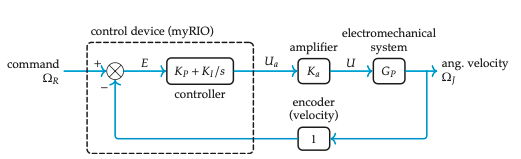
\includegraphics[width=.95\linewidth]{figures/Control-Block-Diagram.png}
	\caption{Control block diagram for the Lab 7 PI velocity-control system.}
	\label{fig:ControlBlockDiagram}
\end{figure}

Starting from the continuous-time controller model,
\begin{equation}
G_C(s) = K_P + \frac{K_I}{s},
\label{eq:gc_continuous}
\end{equation}
and applying the Tustin transformation, the discrete controller can be written as
\begin{equation}
G_C(z) = \frac{U_a(z)}{E(z)} = \frac{b_0 + b_1 z^{-1}}{a_0 + a_1 z^{-1}},
\label{eq:pi_discrete}
\end{equation}
with coefficients
\begin{equation}
a_0 = 1, \quad a_1 = -1, \quad b_0 = K_P + \frac{K_I T}{2}, \quad b_1 = -K_P + \frac{K_I T}{2},
\label{eq:pi_coefficients}
\end{equation}
where $T$ is the sampling period. The discrete velocity error used by the controller is
\begin{equation}
E(n) = \Omega_R(n) - \Omega_J(n).
\label{eq:velocity_error}
\end{equation}

\section{Laboratory Exploration and Evaluation}

\subsection{Problem L7.1}
Design a PI controller for the T1 target system using the root-locus procedure from Sections 7.6.2--7.6.6, then compare the resulting $K_P$ and $K_I$ values with the base gain set computed for this laboratory.

\vspace{\baselineskip}

The base PI gains for the T1a target system are computed from the design relations
\begin{equation}
K_P = \frac{B + 2J\,\mathcal{R}(\psi)}{K_a K_M},
\label{eq:kp_base}
\end{equation}
\begin{equation}
K_I = \frac{Z\left(B + 2J\,\mathcal{R}(\psi)\right)}{K_a K_M}.
\label{eq:ki_base}
\end{equation}

Using the T1a parameters,
\begin{equation}
K_a = 0.06\;\text{A/V},\quad
K_M = 0.0698\;\text{N\,m/A},\quad
J = 7.8\times10^{-6}\;\text{N\,m\,s}^2/\text{rad},\quad
B = 0\;\text{N\,m\,s/rad},
\label{eq:t1a_params}
\end{equation}
the combined amplifier-motor gain is
\begin{equation}
K_aK_M = (0.06)(0.0698) = 0.004188.
\label{eq:ka_km}
\end{equation}

Substituting \eqref{eq:t1a_params} and \eqref{eq:ka_km} into \eqref{eq:kp_base} and \eqref{eq:ki_base}, with the root-locus design selections used for the T1a case, gives
\begin{equation}
K_P = 0.104\;\text{V\,s/rad},\quad K_I = 2.07\;\text{V/rad}.
\label{eq:base_gains_result}
\end{equation}

These values are consistent with the baseline gains reported for Lab 7 and were used as the starting controller settings in the remainder of the experiment. The controller implementation uses velocity in rad/s, which is consistent with the units of the computed gains.

\vspace{\baselineskip}

The base PI gains are $K_P = 0.104\;\text{V\,s/rad}$ and $K_I = 2.07\;\text{V/rad}$.

\subsection{Problem L7.2}
Design a PI controller for your specific T1 target system following the root locus design technique of Sections 7.6.2 to 7.6.6. Compare the gains $K_P$ and $K_I$ to the base set of gains computed in Lab Problem L7.1.

The PI controller for the T1a target system was designed using the root-locus technique described in Sections 7.6.2--7.6.6. From the uncompensated root locus, a gain of
\begin{equation}
K_1 = 0.062
\end{equation}
was selected at the desired pole location
\begin{equation}
\Re(s) = -20.
\end{equation}
A PI compensator with zero location
\begin{equation}
Z_I = -20
\end{equation}
was then introduced. The compensated root locus required an additional gain
\begin{equation}
K_2 = 1.67.
\end{equation}

The resulting PI controller gains were computed as
\begin{equation}
K_P = K_1K_2 = (0.062)(1.67) = 0.10354\;\text{V\,s/rad}
\end{equation}
and
\begin{equation}
K_I = -Z_IK_P = 20(0.10354) = 2.0708\;\text{V/rad}.
\end{equation}

These values were compared with the base controller gains from Problem L7.1.

\begin{table}[htb]
\centering
\begin{tabular}{c c c}
\hline
Gain & Base Gains (L7.1) & Root-Locus Design (L7.2) \\
\hline
$K_P$ & 0.104 & 0.10354 \\
$K_I$ & 2.07 & 2.0708 \\
\hline
\end{tabular}
\caption{Comparison of base and root-locus PI gains for the T1a target system.}
\end{table}

The designed gains are essentially identical to the base gains, with only minor differences due to rounding. Therefore, the root-locus design confirms the controller parameters used for the remainder of the laboratory exercise. A test run of the controller with these gains produced stable closed-loop motor operation.

Steady-state operation in the lab setup was identified using the following observations:
\begin{itemize}
	\item The motor starts and reaches the commanded speed.
	\item $V_J$ settles near the reference value (approximately $99$--$100$ rpm).
	\item $V_J$ does not continually grow, continually decrease, or oscillate wildly.
	\item $VDAout$ settles to a finite value (approximately $150$--$250$ mV) instead of running to the output limits.
	\item The motor sound remains smooth, rather than showing violent oscillation or continuous hunting.
\end{itemize}

The steady-state evidence captured during this test run is shown in Figure~\ref{fig:steady_state_evidence}.

\begin{figure}[htb]
	\centering
	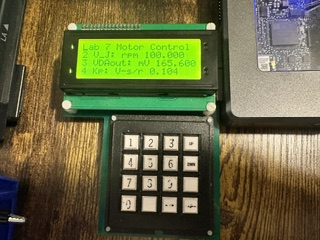
\includegraphics[width=.92\linewidth]{figures/steady-state.jpg}
	\caption{Steady-state controller evidence for the T1a PI velocity-control setup.}
	\label{fig:steady_state_evidence}
\end{figure}

\subsection{Problem L7.3}
Write, test, and debug the program described in Section L7.2. For debugging purposes, use the base set of parameters.

The PI motor velocity controller described in Section L7.2 was implemented in C and tested on the myRIO platform using the base controller gains $K_P = 0.104\;\text{V\,s/rad}$ and $K_I = 2.07\;\text{V/rad}$. Several debugging steps were required to verify proper operation of the velocity measurement, controller calculations, and actuator output. After correcting implementation issues, the controller successfully regulated motor speed. During testing, the measured velocity converged to approximately the commanded speed and the control output remained bounded. As shown in Figure~\ref{fig:steady_state_evidence} (Figure 3), the final implementation exhibited stable closed-loop operation and was used for the remaining laboratory exercises.

The program implementation is available at \url{https://github.com/juliansoh/ME477/blob/main/workspace/Julian_lab7/main.c}.

\subsection{Problem L7.4}
Measure the steady-state speed of the motor with an optical tachometer. Compare this value to the reference speed specified in the table. How close is it?


For this test, the reference speed was set to $V_r = 500$ rpm and the system was allowed to reach steady-state operation before measurement. The program display at this operating point is shown in \autoref{fig:L74_program500}. The optical tachometer readings were between $494$ and $498$ rpm, as shown in \autoref{fig:L74_tach500}. This measured range is very close to the commanded value of $500$ rpm.

\begin{figure}[htb]
	\centering
	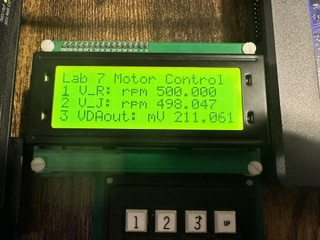
\includegraphics[angle=-90,width=.72\linewidth]{figures/program-500rpm.jpeg}
	\caption{Program display at the $500$ rpm steady-state test condition.}
	\label{fig:L74_program500}
\end{figure}

\begin{figure}[htb]
	\centering
	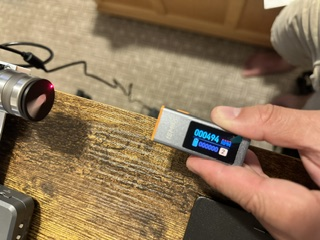
\includegraphics[width=.72\linewidth]{figures/tachometer-500rpm.jpeg}
	\caption{Optical tachometer reading during the $500$ rpm steady-state test.}
	\label{fig:L74_tach500}
\end{figure}

\subsection{Problem L7.5}
While the motor is at steady-state speed, gently apply a steady manual load torque to the motor shaft. What responses do you observe on the display for measured velocity $V_J$ and control voltage $VDAout$? Explain.


While a steady manual load torque was applied to the motor shaft, the measured velocity $V_J$ decreased temporarily. The PI controller responded by increasing the control output voltage $VDAout$. After a short transient, the measured velocity returned close to the reference value while the control voltage remained at a higher level than before the load was applied. This behavior demonstrates the disturbance-rejection capability of the PI controller. The proportional term reacts immediately to speed error, while the integral term removes the steady-state error caused by the applied load torque.

\subsection{Problem L7.6}
Beginning with the base set of parameters, explore the effect of varying the proportional gain $K_P$ on the transient response. Try smaller and larger values of $K_P$. What are the effects on oscillation frequency and damping? Explain in terms of the closed-loop transfer-function parameters described in Section 7.5.2.


The proportional gain was varied while the integral gain was held constant at $K_I = 2.07$. Decreasing $K_P$ produced a slower response with less damping and a longer settling time. Increasing $K_P$ produced a faster response with increased damping and a shorter settling time. This behavior is consistent with the closed-loop transfer function, where $K_P$ appears in the coefficient of the $s$ term and therefore directly influences the damping ratio of the system.

\subsection{Problem L7.7}
Beginning with the base set of parameters, explore the effect of varying the integral gain $K_I$ on the transient responses. Try smaller and larger values of $K_I$. What are the effects on oscillation frequency and damping? Explain in terms of the closed-loop transfer-function parameters described in Section 7.5.2.


The integral gain $K_I$ was varied while the proportional gain was held constant at $K_P = 0.104$. Decreasing $K_I$ resulted in a slower response with lower oscillation frequency and slower error correction. Increasing $K_I$ produced a faster response and a higher oscillation frequency, but it also reduced damping and increased overshoot. This behavior agrees with the closed-loop transfer function because $K_I$ directly affects the natural frequency,
\begin{equation}
\omega_n^2 = \frac{K_a K_M K_I}{J}.
\end{equation}
As $K_I$ increases, the natural frequency increases, causing the system to respond more quickly but with a greater tendency to oscillate. A summary of these observations is provided in \autoref{tab:L77_ki_effects}.

\begin{table}[htb]
\centering
\begin{tabular}{c c c c}
\hline
$K_I$ & Response Speed & Oscillation Frequency & Damping \\
\hline
1.0 & Slower & Lower & Higher \\
2.07 & Baseline & Baseline & Baseline \\
4.0 & Faster & Higher & Lower \\
\hline
\end{tabular}
\caption{Effect of varying $K_I$ on transient-response characteristics.}
\label{tab:L77_ki_effects}
\end{table}

\subsection{Problem L7.8}
Using the base set of parameters, record the control output voltage $U_a$ and measured velocity responses for a step change in reference velocity from $-200$ RPM to $+200$ RPM. In MATLAB, compare these experimental responses with the analytical responses for the continuous-system approximation (see the Lab 7 Appendix summary of the closed-loop model).

The theoretical responses can be calculated using the appropriately scaled MATLAB \texttt{step()} command. Plot the analysis over the experimental responses, and use \texttt{subplot()} to place both the control-value and measured-velocity plots on the same page. What do you conclude?


For Problem L7.8, we performed the comparison in Python (instead of MATLAB) using the captured dataset in \texttt{data/Lab7.csv}. The measured responses ($U_a$ and $\Omega_J$) were overlaid with the analytical continuous-time closed-loop responses on a two-subplot figure (control on top, velocity on bottom), matching the required analysis format. The resulting comparison plot is shown in \autoref{fig:L78_python_comparison}.

\begin{figure}[htb]
	\centering
	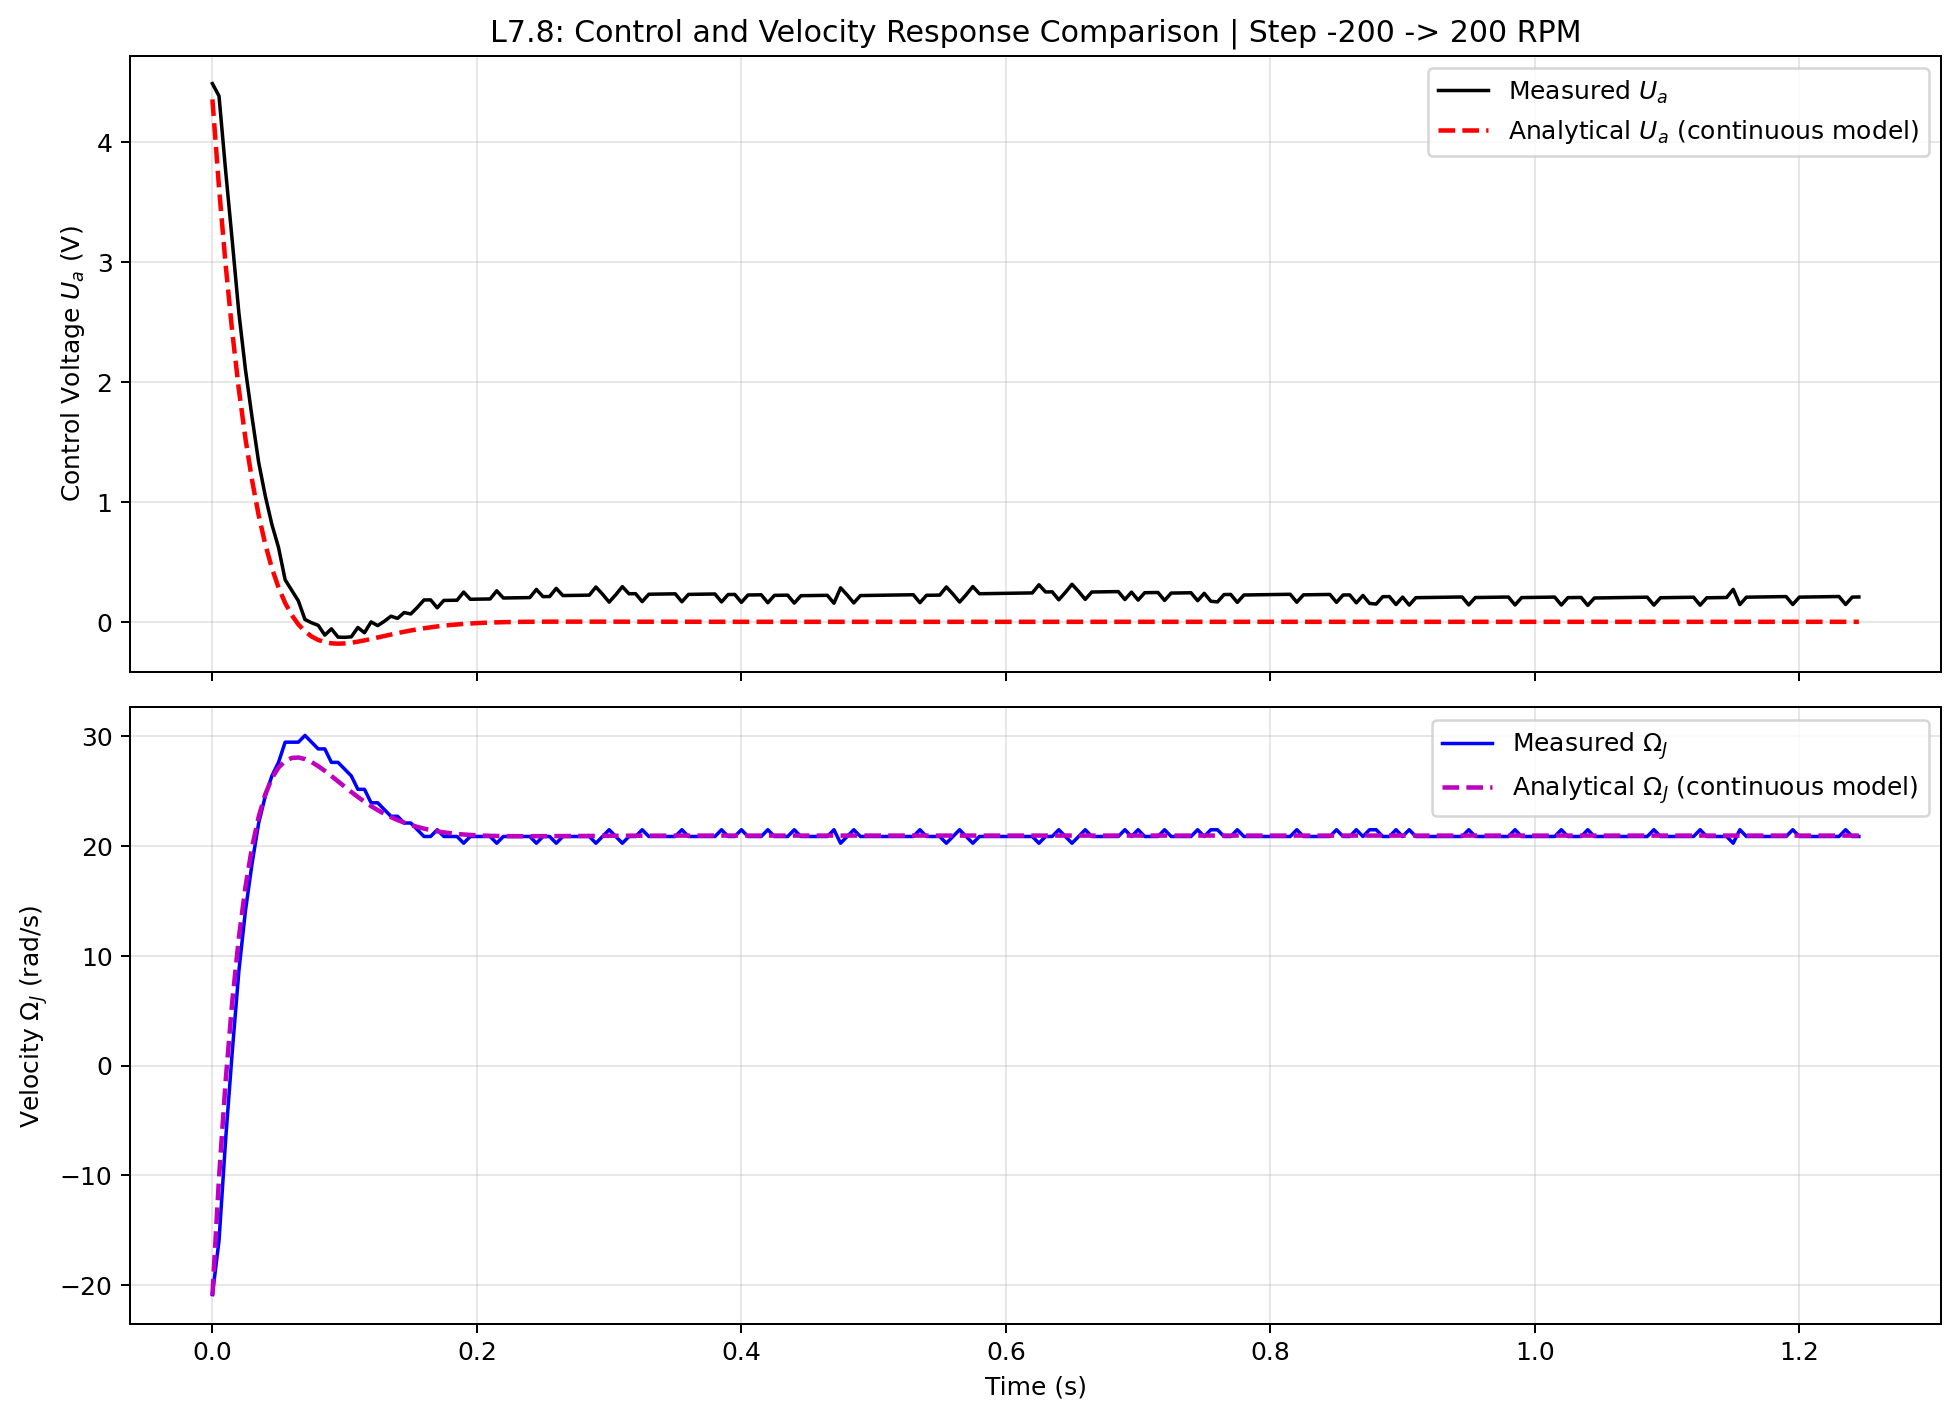
\includegraphics[width=.98\linewidth]{figures/L78-Python-Comparison.png}
	\caption{L7.8 comparison of measured responses from \texttt{Lab7.csv} and analytical continuous-time model responses generated in Python.}
	\label{fig:L78_python_comparison}
\end{figure}

The recorded reference step in \texttt{Lab7.csv} was $-200\,\text{RPM} \rightarrow +200\,\text{RPM}$ with $K_P = 0.104$, $K_I = 2.07$, and $\text{BTI}=5\,\text{ms}$. Quantitatively, the comparison gave a velocity RMSE of $0.7748\,\text{rad/s}$ and a control-voltage RMSE of $0.2351\,\text{V}$.

From the overlaid plots, the measured and analytical velocity responses agree well overall, and the control output shows the same transient trend with small offsets and ripple. The remaining differences are consistent with practical nonidealities such as sampling effects, sensor noise, and hardware limitations.

\section{Author Contributions}

There is only one author for this report and lab.



%%% References -------------------------

\bibliographystyle{plainnat}
\bibliography{report}

%%% Appendices -------------------------

\end{document}  